\section{Faithful Generation}


\begin{frame}{Sequence-to-Sequence Models for Abstractive Summarization (See et al. 2017)}

 \begin{center}
    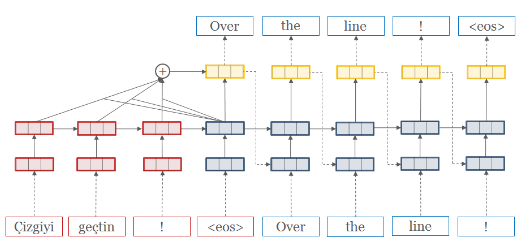
\includegraphics[scale=.5]{images/section4/seq2seq.png}
 \end{center}

 \begin{itemize}
     \item Encoder + Decoder Attention must \textbf{identify important content}.
     \item Decoder must learn to generate fluent  and \textbf{correct} output.
 \end{itemize}
\end{frame}

\begin{frame}{Better Content Selection for Seq2Seq Models}

    \begin{itemize}
        \item Help decoder attention with word importance model:~\\
            \begin{itemize}
                \item Auxilliary Objective to encourage attention distribution
                    to match word importance score distribution. ~\\~\\
        \item Redact or gate words from decoder with low importance.~\\~\\
   \item Training word importance model end-to-end with seq2seq model.~\\~\\
            \end{itemize}

    \end{itemize}

\end{frame}

\begin{frame}{Hallucination in Seq2Seq Models}


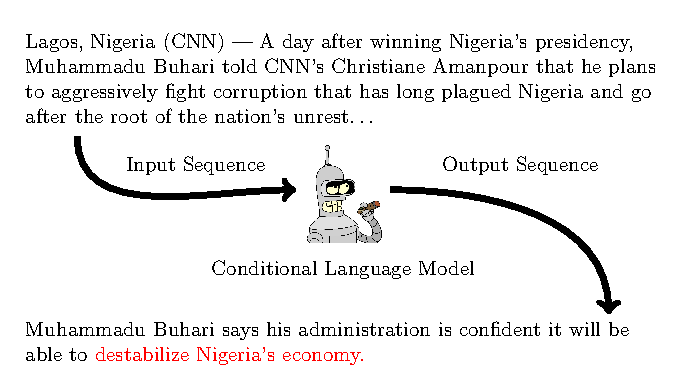
\includegraphics{4_fg/image_texs/clm/clm.pdf}


\end{frame}

\begin{frame}{Faithful Generation}



{\centering
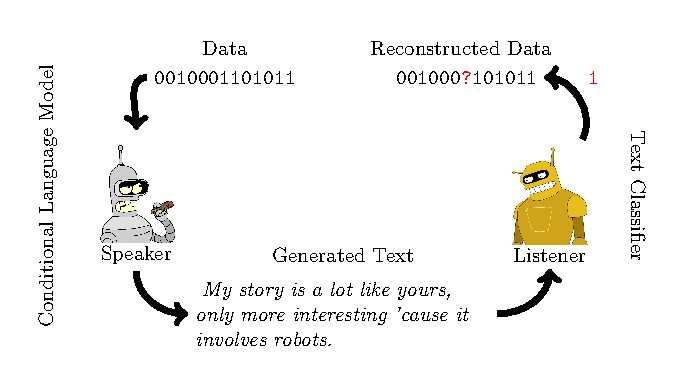
\includegraphics[scale=.7]{4_fg/image_texs/intro_pic/intro_pic.pdf}\\
}
%
\includegraphics[scale=.2]{images/section4/listener.jpeg}
%
\includegraphics[scale=.045]{images/section4/speaker.jpg}
\only<1>{ 
    Motivation:
\begin{itemize}
    \item The speaker generates an utterance from input data.
    \item The listener tries to reconstruct the input data.
    \item The speaker learns directly from the listeners feedback, 
        ensuring that it prefers output likely to be true (w.r.t. the input data).
\end{itemize}
}
%\only<2>{
%Motivation:
%\begin{itemize}
%\item Augment mle training with RL objective to improve accuracy of reconstruction without hurting fluency.
%\item We can apply this object to entire beam search to encourage diverse but accurate generation outputs.
%\item We can use the listener to give our confidence in the correctness of outputs.
%\end{itemize}
%}
%\only<3>{
%Other possible applications: controllable text generation.
%}

\end{frame}


\begin{frame}{Faithful Generation Training}
    Given pairs of input data $x$ and output text $y$: ~\\
    \begin{itemize}
        \item<1-> Pre-train the speaker to generate text from 
            input data: \alert{$\max p(y|x)$}.~\\~\\
        \item<2-> Train listener to predict input from from text $y$: \alert{$\max q(x|y)$}.~\\~\\
        \item<3-> Augment maximum likelihood objective with auxilliary objective
       to maximize the correctness of the input reconstruction under the
            listener: \alert{$\max \mathbb{E}_{y\sim p(\cdot|x)}[ q(x|y)]$}.~\\~\\

\item<4-> We can apply this objective to entire beam search to encourage diverse but accurate generation outputs. ~\\~\\
\item<5-> We can use the listener to give our confidence in the correctness of outputs.
    \end{itemize}

\end{frame}


\begin{frame}{Two Applications}

    \begin{itemize}
        \item \textbf{Data-to-Text}
            \begin{itemize}
                \item Table data $\rightarrow$ text description $\rightarrow$ reconstruct table 
            \end{itemize} 
            ~\\~\\
        \item \textbf{Text-to-Text}
            \begin{itemize}
                \item Document text $\rightarrow$ text summary $\rightarrow$ answer cloze style questions from document
            \end{itemize}
    \end{itemize}

\end{frame}

\begin{frame}{Data-to-Text}
    \centering
    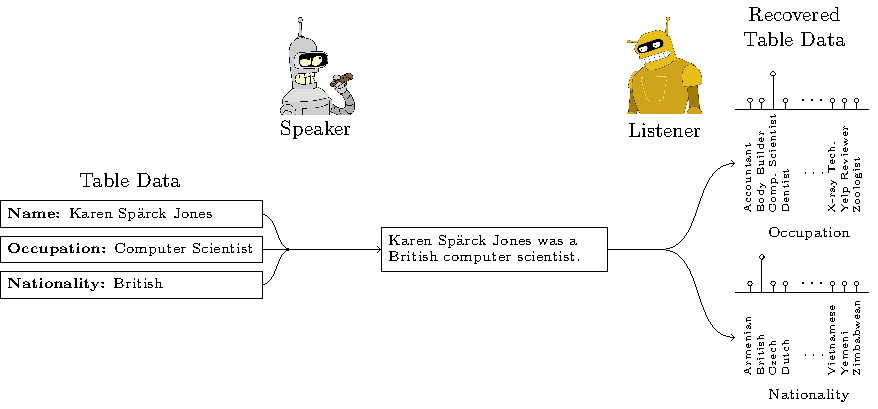
\includegraphics[scale=.8]{4_fg/image_texs/data2text/data2text.pdf}
\end{frame}
\begin{frame}{Text-to-Text}
    \centering
    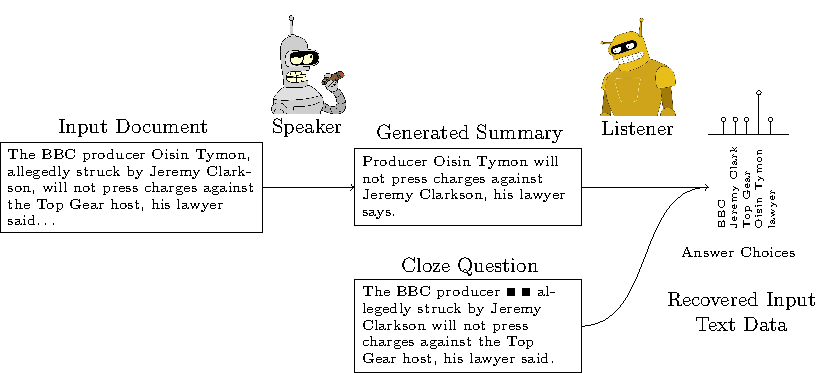
\includegraphics[scale=.8]{4_fg/image_texs/text2text/text2text.pdf}
\end{frame}



\begin{frame}{Planned Experiments}
    \begin{itemize}
        \item Data-to-Text
            \begin{itemize}
                \item<1-> E2E Dataset (Novikova et al. 2017)
                    \begin{itemize}
                        \item Artificially constructed dataset of restaurant data and descriptions
                        \item 50k Meaning Representations/text description pairs.
                    \end{itemize}~\\
                \item<2-> WikiBio Datatest (Lebret et al. 2017)
                    \begin{itemize}
                        \item Biographical data paired with text descriptions,
                            taken from Wikipedia.
                    \item 700k table/text pairs.
            \end{itemize}
            \end{itemize}
            ~\\
        \item<3-> Text-to-Text
            \begin{itemize}
                \item<4-> TL;DR Dataset (V\"olske et al., 2017)
                    \begin{itemize}
                        \item $\approx 4$ million Reddit comments with 
                    summaries. 
                    \item Non-news dataset!
                    \item Comments shorter than news article: possibly easier to generate cloze questions.
            \end{itemize}~\\
                \item<5> Lots of news (CNN/DM, NYT, Newsroom, XSUM)
            \end{itemize}
 \end{itemize}
         \end{frame}

\begin{frame}{Planned Experiments}
    \begin{itemize}
        \item REINFORCE (Williams, 1992) style learning objective to maximize
            correct classification by the listener.~\\~\\
        \item<2-> While incorrect statements in best beam candidate might be rare, errors more likely in remainder of beam.~\\~\\
        \item[$\Rightarrow$]<3-> Optimizing over whole beam should be easier to demonstrate 
            improvements. ~\\~\\
    \end{itemize}
\end{frame}

\begin{frame}{Planned Experiments}
    \begin{itemize}
        \item Interesting angles to take even if performance improvements are not staggering:
            \begin{itemize}
                \item<1-> Apply listener as 
                    beam re-ranking criterion during generation.

                \item<2-> Localize error signals with token level explanations 
                    from classifier.
                \item<3-> Understand correlation in listener models $\Rightarrow$ 
                    enforce independent listener models.
               \end{itemize}


               ~\\~\\
           \item<4-> We can also focus on the cloze question generation aspect.
            \begin{itemize}
                \item Many heuristics for creating cloze style questions.
                \item Incorporate word importance model.
                \item Guided question generation to improve training.
            \end{itemize}

    \end{itemize}
   
    

\end{frame}


